\chapter{Introduction}


% am Ende der alten Intro...
% hier fehlt mir eine klare Beschreibung der Problemstellung...du bist sehr generisch und sagst, dass es vor und nachteile hat, benennst diese aber nicht
% Was auch fehlt ist dein Lösungsvorschlag bzw. deine Idee, wie man die Problemstellung bearbeiten kann (was du in dieser Arbeit vorhast)



% \section{Problem Statement}

% 1. Absatz: Beschreibe uns das Forschungsfeld in dem du dich befindest (DevOps / GitOps)

Increasingly more organizations are adopting 
a DevOps culture
\autocite{devopsCultureSanchez2018characterizing}
to develop new applications and services at high velocity. 
After all, a culture that encourages
shared responsibility, communication, transparency,
and continuous and immediate feedback,
helps to narrow the gaps between teams and thus accelerate the development process.
In order to
reduce friction between engineering teams who are involved in the software development lifecycle (SDLC),
a practice called GitOps has emerged.
It allows developers who are already familiar with the version control system Git,
to easily deploy their applications to target environments in a self-service model.
All sorts of IT infrastructure can be managed, purely by
interfacing with declarative state definitions stored in Git.
%
84 percent of organizations that have embraced cloud native technologies
have adopted practices and tools that adhere to GitOps principles
\autocite{scalingGitOps2023weaveWorks}
\autocite{cncfAnnualSurvey2022}.
%\enquote*{GitOps principles are 4x as likely to be followed at mature cloud native organizations, versus those that have not embraced cloud native techniques.}
%\autocite{cncfAnnualSurvey2022}

%GitOps is a set of principles for operating and managing software systems.
%These principles are derived from modern software operations, but also have their roots 
%in existing and widely adopted best practices. 

% 2. Absatz: Beschreib uns das Problem bzw. die Challenge in diesem Forschungsfeld (Was ist die Problemstellung, die es zu bearbeiten gilt)

% why is it important to solve the problem?

GitOps as a practice for deploying and managing software systems has an unresolved problem, which is
the process of promoting releases between multiple deployment environments.
%(fig. \ref{fig:releasePromotionProcess}).
%
%\begin{figure}[h]
%	\centering
%	\fbox{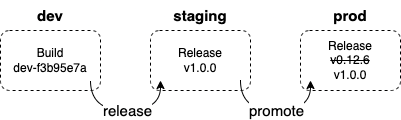
\includegraphics[width=.70\linewidth]{figures/release-promotion.drawio.png}}
%	\caption{Promotion between environments.
%		%		(\citeauthor{ref}, \citeyear{ref}).
%	}
%	\label{fig:releasePromotionProcess}	
%\end{figure}
%
Current GitOps tools do not provide an integrated solution for this process,
nor do they provide any sort of abstraction for defining environments.
Promotions are often achieved via hard-coded file copy operations,
which is done manually or with a workflow/pipeline system.
Furthermore, for each configuration/templating tool which is used,
the modeling of different deployment environments, as well as the
process of promotion, is unique.
This results in the process of promoting releases with GitOps
not being a streamlined task.
%Clear guidelines and best practices,
%as well as tools which implement them,
%are missing in the GitOps ecosystem.
A GitOps-native way for doing automated promotions between environments is
not provided by the currently available open-source tools.

% 3. Absatz: Was schlägst du vor, wie man die Problemstellung bearbeiten könnte? Beschreibe uns deinen Lösugnsvorschlag dieser Arbeit, wie man das Problem bearbeiten könnte

%
The given problem could be addressed by
providing standardised models 
for defining deployment environments and promotion processes.
%
An application programming interface (API) extension for Kubernetes,
namely a custom resource definition,
could provide abstract representations for these models.
%
This would allow users to define
their environments,
and how they want releases to be promoted between them.
%
Additional logic could be introduced into the promotion process,
like specifying a rule which ensures that new releases must first pass
certain environments or other objectives before being promoted to production.
%
The abstraction would also enable transparent replacement of the
configuration or templating tool,
while keeping the desired state definition intact.
%
Following the principles of GitOps,
an operator would ensure the continuous reconciliation
between the desired and the actual state of the resources.

% 4. Absatz: gib uns einen Ausblick (Paint the Big Picture) wie deine Lösung mit dem großen Ganzen zusammenhängt

%
The proposed solution of the problem should
present a possible way of defining environments and promotion processes abstractly,
onto which future work could build upon.
%
Additionally the solution should
provide a protoype of a toolkit,
which could serve as an optional component
in addition to existing tooling.
%
Solving the problem of release promotion natively within the GitOps toolkit,
would make the adoption of GitOps more appealing,
especially for organisations, which have the need for many different environments.
%
As a result
this could generally accelerate the widespread use of GitOps
and thus enable more organisations to develop higher quality software.
%










